\section{Protocol communication}\label{cha:protocolDesign}
\todo{be more humble, analytic and include possibilities or explain why omitted}
To transmit the data from the nodes to the main node, a protocol must be implemented.
The protocol must support the utilized hardware components and be designed to work within their limitations. 

% Background/meta
The protocol to be developed for the solution will be based on the networks examined in Section \ref{fig:topologies} and the protocols described in Section \ref{cha:comprot}.
There are a number of considerations to be made to develop a protocol that complies to the requirements.
Because the sensor nodes are battery driven, most of the choices are done with power consumption as a priority, to increase the battery longevity.

% Range limitations
While the individual nodes have a relatively short communication range, a network of these devices can have a longer reach if the nodes are able to relay data through each other.
Therefore, relaying must be supported by the protocol as stated in \ref{cha:requirements}. 
Another restriction of the radio modules is their range. The reach of the system can be extended by introducing relaying, so that a sequence of nodes can interconnect and transfer data through the branch in the tree. 

% Other limitations and considerations
%To fulfill the requirements found in \ref{cha:requirements}, there is no demand to request data for only one specific node at a time.
There are multiple methods to request data from the network nodes, some of the most used ones can be found in \ref{cha:comprot}. \todo{research}

The radio modules selected for the solution are half-duplex\todo{ensure duplex is described in theory} and not capable of full-duplexing, and this limitation needs to be addressed in the development of the transmission part of the protocol. 

% Already mentioned in design intention/data handling => move?
For power consumption and complying to the usage, the network nodes are controlled by the main node, and the nodes will transmit sensor data on demand.
This implementation will keep the nodes in a low power listening mode until a data request is received.
The nodes transmitting their sensor readings automatically requires some sort of synchronization, so the node data is updated for every node and transmitted back to the main node.
There is no requirement for real-time monitoring of the golf course, making it difficult defining a data transfer interval that matches both power consumption as well as the need for information.
Hence, an on-demand request for data will be sufficient.

\subsection{Transfer method and topology}\todo{new title}
% Intention/motivation
The solution is required to gather sensor data from all nodes in the network, and this subsection will contain the considerations regarding choice of method and the according topology.

%This enables the main node to broadcast data requests throughout the sensor network, and likewise transmitting data readings from the sensor nodes to the main node.

% The two types of communication (data request and data respond)
As the sensor readings are required on-demand, there must be at least two types of communication. The first being the data request, an outgoing signal from the main node, notifying the data demand. This is a broadcasted packet, as every node is targeted as recipient. The second type is data response, while the sensor readings needs to be returned to the main node for storage and representation. The design of the two types follows.

% Design of data request: individual request
One data gathering method is to demand data explicitly from each node. That can be done by transmitting a unique data request to every node in the network, addressing each nodes by its identification. This would require the main node to create an individual request to each node in the network, and the network nodes to know the path through the network to the addressee, so that the request can be relayed correctly. This is not appropriate as routing tables would use a significant amount of the network nodes' limited memory\todo{how much would routing tables fill?}. In case of disconnected nodes, the routing tables must be reconfigured, to make sure packets are relayed in a path that actually exist. This would accordingly require nodes to somehow broadcast that they are still alive, and thereby consume more energy in addition to more memory.

% Design of data request: broadcast request
Another method of data gathering is by a request broadcast. This would work as a flooded request throughout the network.
A data request will be broadcasted to all nodes in the network, using flooding, and will only require one unique packet. 
If the broadcast is done by controlled flooding, there will be no cycles, and the outgoing transmit topology will consequently be a tree. 
Flooding will only handle one packet, but the nodes can receive the same packet multiple times and must analyze and discard any duplicate packets.

% Data request method selection template
The protocol selected for the solution is partly based on the flooding protocol.
This protocol is a method where the data request can be transmitted by flooding the network, without needing to send a tailored request to every node in the network. 

The controlled flooding has a low memory impact and thus best suited for the solution. The flooding protocol will create a tree which can be utilized to create a return path for the nodes' sensor readings.

% Practical implementation of data request
\begin{figure}[h!]
	\centering
	\makebox[\textwidth][c]{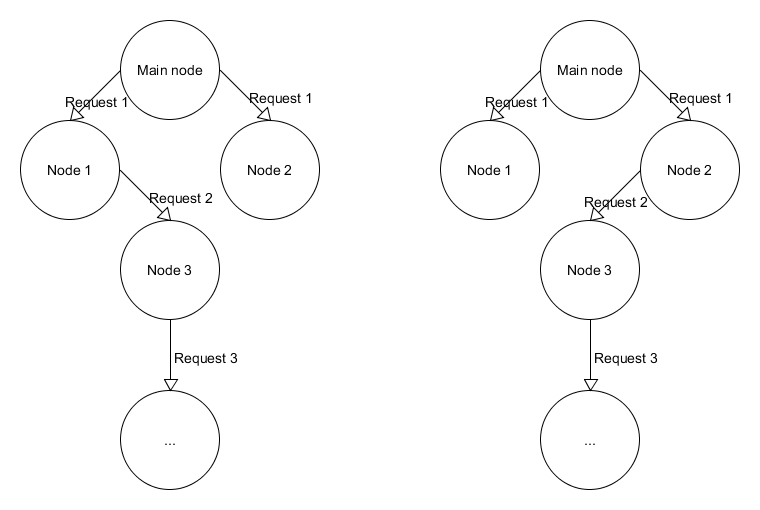
\includegraphics[scale=0.4]{chapters/design/figures/branchExample.png}}
	\caption{The tree's structure can vary depending on the node that connects to the main node first.}
	\label{fig:treeVariation}
\end{figure}


The tree created in each request broadcast can vary in its structure, depending on interference, removal of nodes or faulty nodes or by other occurrences. \figref{treeVariation} shows an example of how the tree can vary: first the main node will broadcast "request 1", which is received by both "node 1" and "node 2". An external node in the system will always handle its own sensor data before it starts relaying data from other nodes. If the main node receives data from "node 1" first, then the resulting tree will match the tree seen to the left on \figref{treeVariation}. If "node 2" connects to the main node first, then the tree will match the tree on the right.
This will effectively solve the requirement of responding appropriately to a disconnecting node, as well as including new nodes in the network, since a new tree is constructed with each wave of requests from the main node.
It will also use the shortest path to every node, due to each node connecting to its immediate neighbors.

% Design of data respond
The tree instantiated by the flood, can be used to create a path from each node to the main node.
The receiver of a request signal can use the sender as the parent when data is to be returned.
The child will then repeat the request signal, and be the parent of nodes hearing it.

% Topological consequence of data communication: tree
The topology of the network will effectively be a tree, although prone to changes in branches.
Any node receiving a request signal will then be able to respond to its parent, causing all nodes to have a single identifier for the routing towards the destination node, the main node.

\subsection{Sequence}
The protocol sequence is determined as the following. A flowchart can be seen in the appendix.\todo{add flowchart to appendix}

This is the operation structure for each individual node in the system.
\begin{enumerate}
	\item Receive data request (Wireless request for nodes, user input at the main node)
	\subitem Ignore if (already received or not recipient of package)
	\item Remember parent (MN skip)
	\item Acquire sensor data
	\item Send sensor data to parent (if silence?)
	\item Receive acknowledgment of sent package
	\item Send data request to all
	\item Receive data from children
	\item If no response or acknowledgment within 10 min: (deep) sleep?
\end{enumerate}

\subsection{Interference handling} \label{cha:crcDesign}
When utilizing wireless communication, interference can be a problem, as explained in section \ref{cha:floodingSec}. This is also the case when using controlled flooding, but using a protocol can help reduce problems with interference, for instance by validating the transferred data and acting accordingly.

Interference might change packets, which makes it impossible to use the received data. Figure \ref{fig:prottree1} shows an example of a possible interference scenario, where nodes 5, 6, and 7 could send packets at the same time, causing node 3 to receive scrambled data.

To ensure this is not a problem, a checksum is used for verifying packets. This checksum is transmitted with the data and recipient. When a node receives a packet, this checksum is calculated, and compared to the one in the packet. How the checksum is calculated were explained back in \ref{cha:crcComp}.

To ensure that a packet with the correct checksum will arrive at some point, the nodes will wait a random, but longer, interval between attempting to send data. This means that at some point, the data will be transmitted to the receiver without interference. \todo{add ref}
This is possible, as time is not essential, and the delay between trying again is short.\todo{time is not essential?}


\subsection*{Example}
The protocol uses flooding to distribute the data request through the network. 
When data is requested by the user, the main node sends a packet containing a sensor reading request. 
The nodes that receive this packet directly from the main node is the first level of nodes in the tree, as seen in figure \ref{fig:prottree1}. 
These nodes then read the moisture values from their sensors and transmit these back to the main node. 

The first level nodes then request data from the nodes within their range. 
The nodes receiving this request firstly verifies that it is a new request, then registers the node that requested data as its parent. 
These nodes are second level nodes. The second level nodes read from the sensors, and sends data back to their parents. The parents then relay the data to the main node. 
This procedure continues until all reachable sensors have relayed data back to the main node.
An illustration showing an example of a tree is seen on Figure \ref{fig:prottree1}.

For each new data request from the main node the tree structure and node levels are assessed again as they might have changed, due to new or disconnected nodes.

\begin{figure}[!h]
	\centering
	\makebox[\textwidth][c]{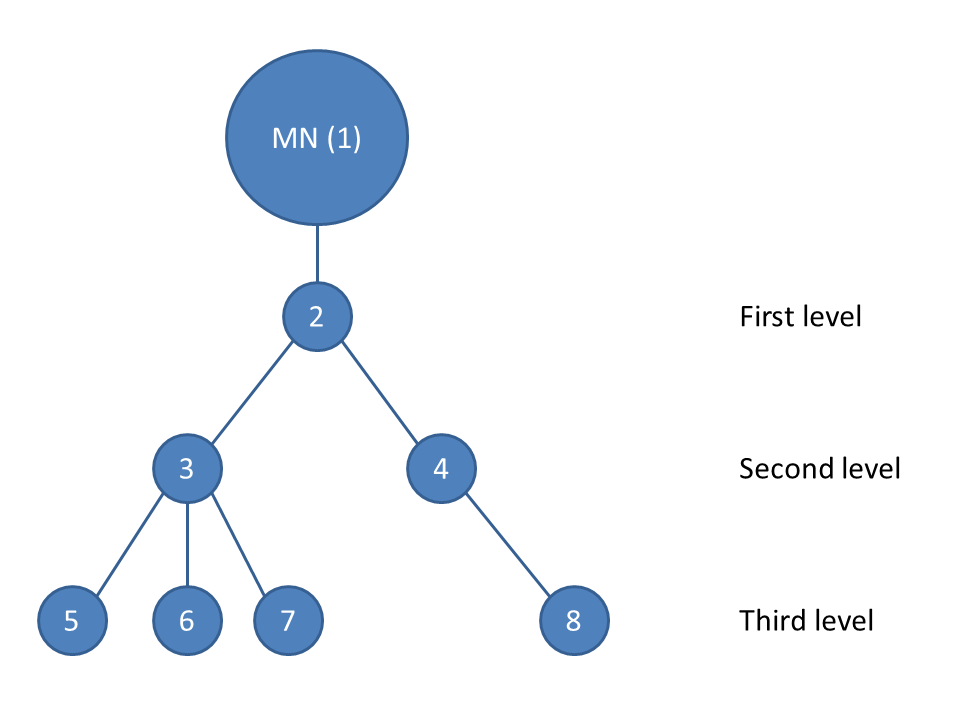
\includegraphics[width=1\textwidth]{chapters/design/figures/prottree1.png}}
	\caption{Example of a tree.}
	\label{fig:prottree1}
\end{figure}








\section{Protocol packet}
This section covers the descriptions and decisions regarding the packets in the system.


\subsection{Packet types}
There are multiple types of data needed to make a functioning protocol. The nRF24L01 supports data payloads up to 32 bytes, and is accordingly the limit of data to transfer in each packet.
Although, a decrease in amount of data can enable the protocol to be implemented on more limited hardware in addition to use less energy on broadcast.

There are seven types of packages: error, data acknowledgement, data request, data, pair request, pair request acknowledgement, and clear signal.
These are used to tell the receiver what kind of data the packet contains, so that the receiving node can decide how to handle the received packet. 1 byte will be sufficient to store the packet type.
Below is a description of the packet types:


\textbf{Error}\newline
Packets are not always transferred correctly, and this is why a node will verify the integrity of a packet whenever a new packet is received. Section \ref{cha:crcDesign} describes how this is done. If the checksums do not match, then the type of the packet will be set to \textit{error}. If the radio module is listing and in the time do not received a packet, it will also return an \textit{error} packet, discarding it.

\textbf{Data request}\newline % Mention lifespan?
To signal that a node is ready to receive data, it will broadcast a \textit{data request} packet to all sensor nodes within range.
Each sensor node will then respond with a \textit{data} packet, containing their sensor data, before they create and send a new \textit{data request} packet out though the network.
The packet contains the id of the node transmitting it, so each sensor node receiving the packet, knows where it comes from.

\textbf{Data}\newline
A \textit{data} packet is a response to the \textit{data request} packet.
A sensor node which receive a \textit{data request} will transmit a packet with data back to its parent.
The parent is whom the \textit{data request} came from.

\textbf{Data acknowledgement}\newline
A \textit{data acknowledgment} packet is expected to be received after a \textit{data} packet have been delivered. 
When a node requests data from the surrounding nodes, they will all start responding by sending their \textit{data} packets, which cause a great deal of interference. The \textit{data acknowledgment} is used to confirm that the sent \textit{data} packet have been received correctly by the node that requested the data.

\textbf{Pair request}\newline
A \textit{pair request} packet is sent from a sensor node directly to the main node. The purpose is to have each sensor node registered in the system and have the main main node generate and assign an ID. This enables the main node know when all data is collected at the end of a wave of \textit{data requests}, and to differentiate the collected data.

\textbf{Pair request acknowledgement}\newline
The \textit{pair request acknowledgement} packet is sent by the main node and used to confirm that the \textit{pair request} has been received and accepted. A \textit{pair request acknowledgement} packet also contain the assigned ID that have been assigned to the specific node. When the two nodes, main and sensor node, are paired, can the sensor node then be deployed in the field as a park of the network. 

\textbf{Clear signal}\newline
The \textit{clear signal} is used to reset every node in the network, which will happen once the main node have received data from all registered nodes in the system.
The \textit{clear signal} packet let every node in the network know that it should forget any previous information stored, except its own ID, such as parent information. This is done to add flexibility to the system. When \textit{data request} spread through the network, it forms a tree based on how the nodes are placed. By resetting with the \textit{clear signal}, a new tree is created each time a new wave of \textit{data requests} goes through the network, which in turn means that nodes can be moved around the golf course between waves of \textit{data requests}. How the trees are constructed was explained in section \ref{cha:crcDesign}.


\begin{figure}[h!]
	\centering
	\makebox[\textwidth][c]{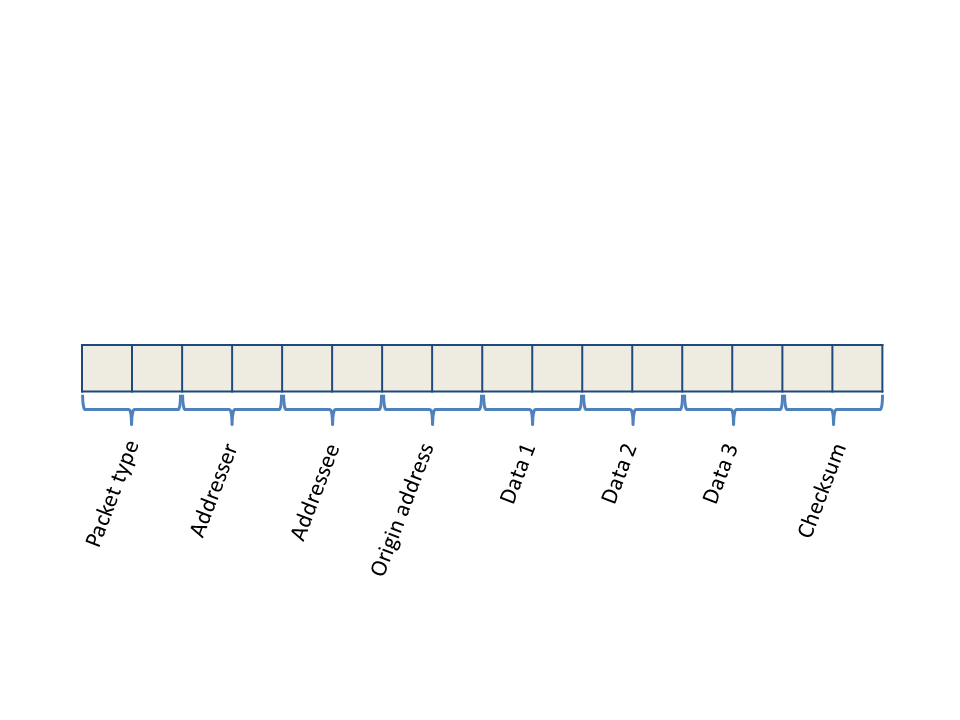
\includegraphics[width=1\textwidth,trim={0 3cm 0 8cm},clip]{figures/dataalloc.png}}
	\caption{Data allocation in packets.}
	\label{fig:dataalloc}
\end{figure}

\subsection{Addresses}
Twelve bytes have are used to keep track of a packet. These contain the addresser, addressee and the origin address which can be seen on figure \ref{fig:dataalloc}. 

\textbf{Addresser}\newline
When a node receives a packet, for instance a packet of the data request type, the node in question need to respond with its sensor data. The node could begin broadcasting its sensor data openly as response, however this could potentially be received by other nodes in range, whereas the sensor data might be irrelevant. This is why a packet contain the id of the sender, which is the addresser. This gives the node knowledge of the node that requested data and can therefore address its data correctly. Other nodes in range might receive the data as well, but they will ignore the this packet since it was not addressed for them.

The addresser field of a packet will change during the packets lifetime. This happens when a node forwards a packet from another node. The addresser id be replaced by the id of the node relaying the data.

\textbf{Addressee}\newline
When a node wants to send a packet with its sensor data, a data type packet in this case, it need to specify who this data is meant for, which is the node that requested the data. The id of the node that requested the data will be marked in the packet as the addressee. This is done to ensure that the packet reaches the intended node. When a node, that are expecting a data packet, receives such a packet, it compare the addressee of the packet with its own id. The packet will be ignored by the node if the addressee and id does not match.

The addressee field of a packet will change during the packets lifetime. This is the case when the packet is relayed, in the same way that the addresser changes.

\textbf{Origin address}\newline
The origin address contains the id of the node where the data of a specific packet originated. This data is used by both the main/central node and the external nodes to differentiate the data.

The origin address field of a packet will not be altered during the packets lifetime.


\subsubsection{Data}
When a data packet is constructed, the sensor data is stored in the "data" fields of the packet as seen on figure \ref{fig:dataalloc}. There are three fields available for sensor data storage. The solution will at this time only contain an implementation of the moisture sensor, but the aim of the three data fields is to add extendability by enabling support for a maximum of tree sensors per node, each with its own field in the packet.


\subsubsection{Checksum}
There is a possibility that a packet is not transferred correctly. This could be due to interference. The packets checksum is stored in the checksum field of the packet and is used for verification. Interference handling was discussed in section \ref{cha:crcDesign}.


\subsubsection{Packet allocation}
The limitation of the network size is 1000 nodes. This means the addresser, addressee and origin address fields need to support 1000 unique addresses, which requires 9 bits. The allocated size for the addresses are accordingly 2 bytes(16 bits) each to maintain usage of whole bytes. This is done because it is more efficient to manipulate a byte instead of a bit \cite{bytevsbit}. The addresses requires 6 bytes in total.

The readings of the moisture sensor have a resolution of 1024 values, and the required size allocated for the sensor reading data is 10 bits. The allocated data size in the transfer is therefore 2 bytes.

To verify the integrity of the received package, a Cyclic redundancy check (CRC16) is appended. CRC16 uses 2 bytes to distinguish a successfully transfered packet from an erroneous one. 

The sizes of the different data to transfer sums up to 16 bytes and the distribution is displayed in \figref{dataalloc} as the data 1, data 2, and data 3 fields.




\subsection{Verification of a packet}
%Verification of a message
The received packet is verified by doing one of the two following methods. 

Generate checksum of message m and compare with received checksum r.
The checksum of a correctly transferred packet $T$ is 0, because a package $T$, if correctly transferred, is some quotient $Q$ times the polynomial $G$, as seen in eqref[earlier]. If a division has a zero remainder, the packet was transferred correctly.




\subsection{Adding and removing nodes}
If a new node is to be added to the network, it needs an identifier in the system so that its sensor reading can be recognized. The identifier is permanent as long as it is in the network.
The identifier is provided by the main node by pairing the device with the main node before adding it to the network. 

The identifier is used to address parent nodes to relay the packets when transmitting sensor data. In figure \ref{fig:prottree1}, the nodes 5, 6, and 7 would send and address packets to the parent by the identifier 3. This means that other nodes in the vicinity would ignore these packets, and only node 3 reacts on the packets. Node 3 would then relay the data to node 2, as 2 is 3's parent, and finally 2 would relay to MN.

Should a node somehow disconnect from the network, the nodes connected to this node will receive the packets from another node first, and from that point on use that as the parent. This is if there are any nodes in range of the disconnected nodes' subnodes. 

\begin{figure}[!h]
	\centering
	\makebox[\textwidth][c]{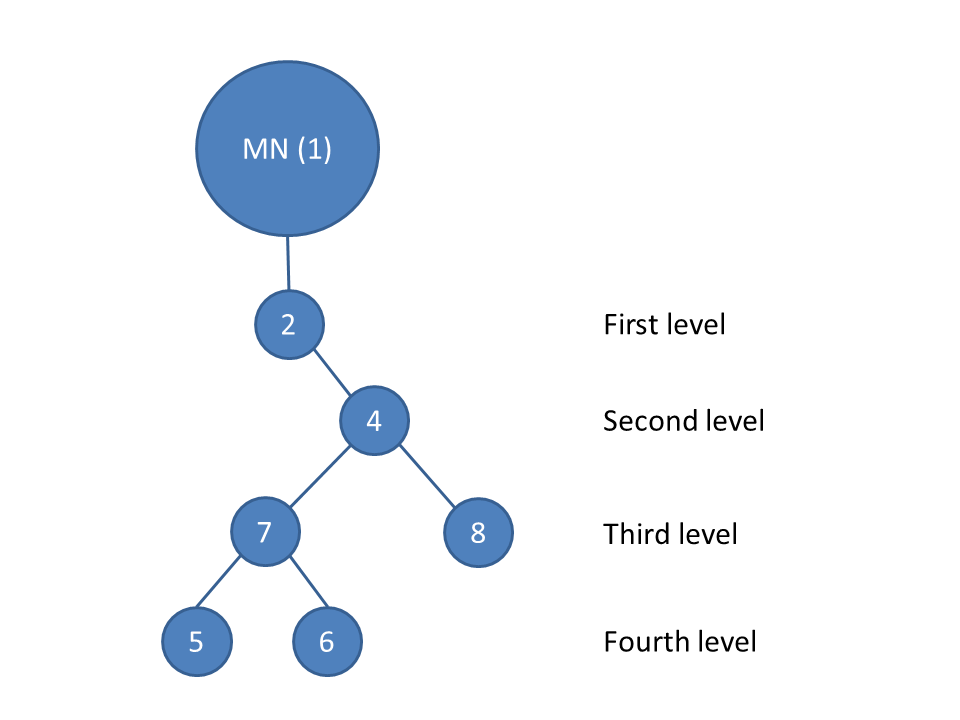
\includegraphics[width=0.8\textwidth]{chapters/design/figures/prottree2.png}}
	\caption{Example of a where node 3 disconnected.}
	\label{fig:prottree2}
\end{figure}

An example of this can be seen on Figure \ref{fig:prottree2}. This figure shows how node 3 disconnected, and now node 7 is attached to node 4 instead. This, of course, assumes that node 7 was in range of node 4.
This means that the next time data is requested, node 7 will be the parent for node 5 and 6, and they will now be a level higher than before.
